\documentclass[10pt, compress]{beamer}

\usetheme{m}

\usepackage{booktabs}
\usepackage{amsmath,amsfonts,amsthm,commath,bm}
\DeclareMathOperator*{\plim}{plim}

\title{Potentials and Perils of Preprocessing}
\subtitle{Alexander W. Blocker and Xiao-Li Meng}
\date{\today}
\author{Maxime and Angela}


\begin{document}
\maketitle

\begin{frame}[fragile]
    \frametitle{Overview of the Paper}
    
    Addresses data preprocessing and its effect on later analysis in three main ways:
    \begin{enumerate}
    \item Points out potential problems with current preprocessing strategies
    \item Describes a statistical framework for analyzing data preprocessing
    \item Proves some theorems about sufficiency 
    \end{enumerate}

\end{frame}

\begin{frame}[fragile]
    \frametitle{What is the Preprocessing problem?}
  
  \begin{center}
    \textbf{Preprocessing} constrains downstream data analysis, 
    
    particularly in \textbf{multiphase inference}:
  \end{center}
  
    \setbeamercovered{transparent}
    \begin{enumerate}[<+->]
    \item Original data is processed at each level of the analysis pipeline, often irreversibly, based on assumptions about what the future analysis may be and the observation mechanism
    \vspace*{5mm}
    \item Even if original data were passed down, many users may not know how to process the data themselves- the analyst performing the preprocessing may have detailed knowledge about the experimental situation
  \end{enumerate}
  
\end{frame}

\begin{frame}[fragile]
    \frametitle{The Multiphase Setup}

    Two phases:
    \begin{enumerate}
    \item \textbf{Preprocessing} = Data generation, collection, preprocessing
    \item \textbf{Downstream Analysis} = inference using output from phase 1
    \end{enumerate}
    
    \begin{figure}[h!]
    \centering
    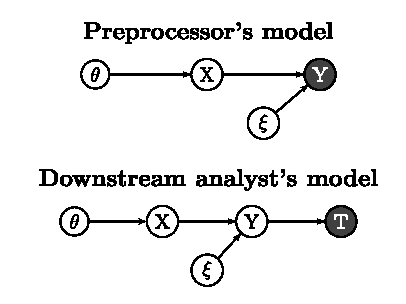
\includegraphics[width=.6\textwidth]{assets/two_phase_setting.ps}
    \end{figure}

\end{frame}

\begin{frame}[fragile]
    Do we want another slide here? basic notation or definitions, discussion of the missingness and missingness pattern?

\end{frame}

\begin{frame}[fragile]
    \frametitle{Square Kilometer Array}
    \begin{columns}
        \column{0.5\textwidth}
            \begin{itemize}
                \item Radio telescope to be built 2018-2030
                \item Total collecting area = $1~\mathrm{km}^2$, bet
            \end{itemize}
        \column{0.5\textwidth}
            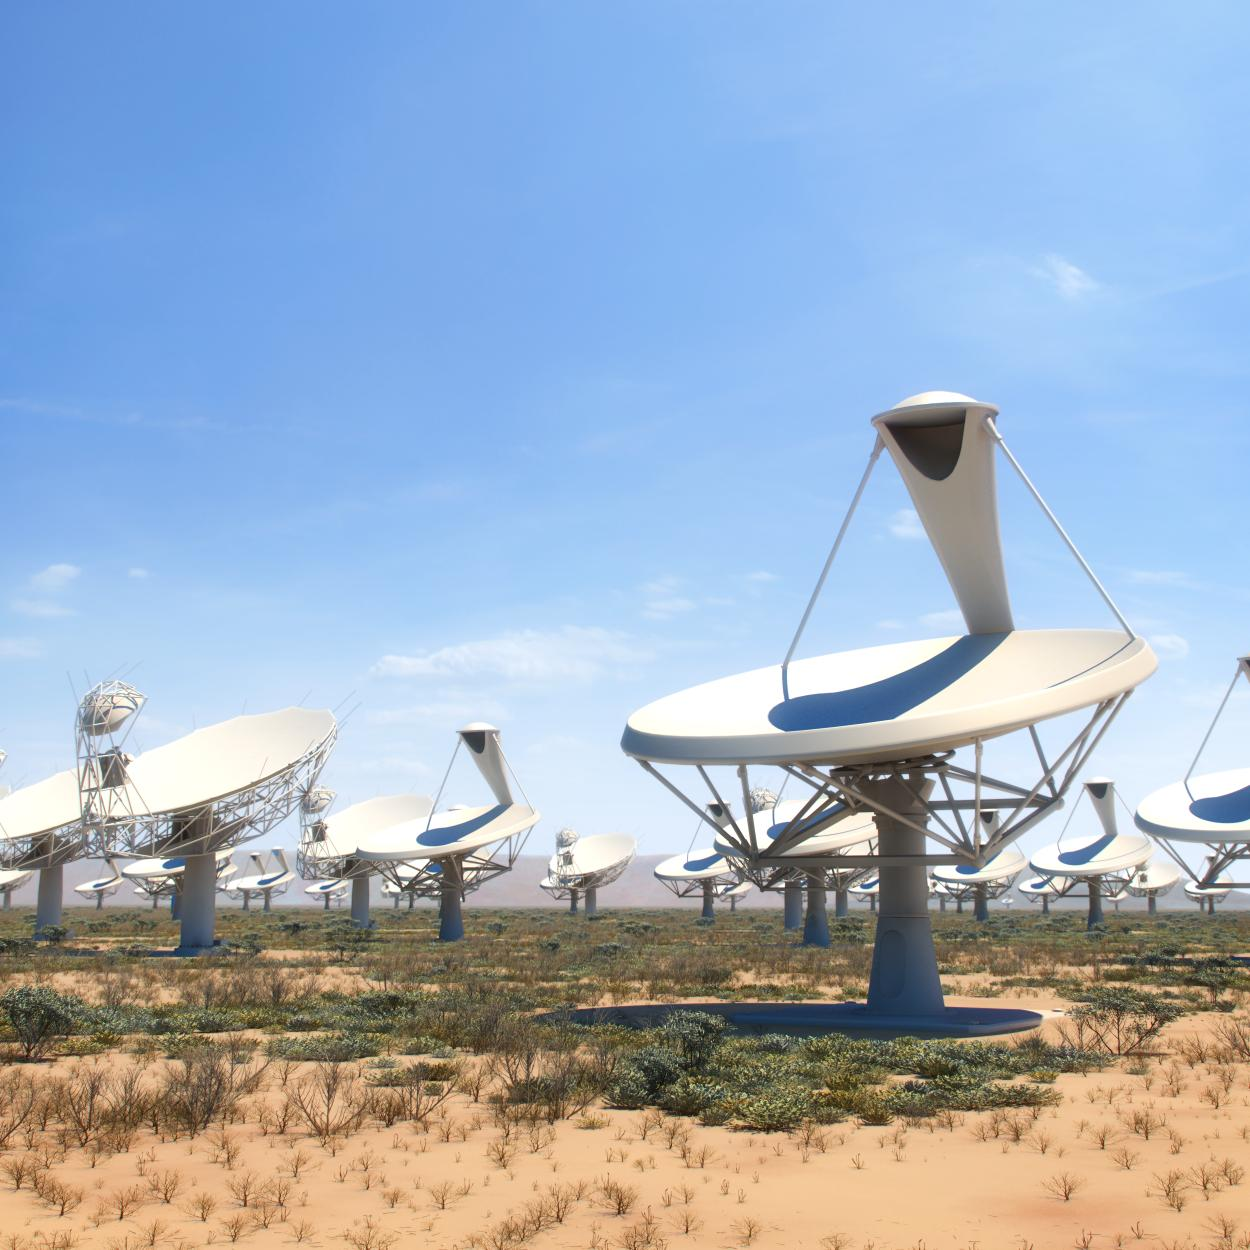
\includegraphics[width=\textheight]{assets/ska_dish_mid_africa_closeup.jpg}
    \end{columns}
\end{frame}

\begin{frame}[fragile]
    \frametitle{High-throughput Biology: Expression Microarrays}
    
    \textbf{Raw data} = probe intensity measurements with control probes, but \textbf{want to study} log fold change in gene expression
    
    \textbf{Many levels of preprocessing:} 
    \setbeamercovered{transparent}

    \begin{enumerate} [<+->]
    \item \textbf{background correction} to reduce noise- many different algorithms, mostly passing down point estimates
    \vspace*{5mm}
    \item \textbf{normalization across different microarrays} to reduce systematic error- but can compromise inferential validity if data is used for other analyses
    \vspace*{5mm}
    \item data transformations, screening for data corruption, etc.
    \end{enumerate}
    
    At each step of preprocessing, large amounts of information are lost

\end{frame}

\begin{frame}[fragile]
    \frametitle{What should we retain?}
    \begin{itemize}
        \item \textbf{Optimal:} lossless compression to \textbf{minimal sufficient} statistic for a given research model
            \begin{itemize}
                \item Sufficiency: $\Pr\del{\theta \mid Y,T\del{Y}}=\Pr\del{\theta \mid T\del{Y}}$
                \item This is only practical if the analyst's model $X \mid \theta$ is specified and known before preprocessing.
                \item \textbf{More realistic:} Hope downstream analyst's scientific model is related (congenial) to preprocessor's observation model
            \end{itemize}
    \end{itemize}
\end{frame}

\begin{frame}[fragile]
    \frametitle{What should we retain?}
    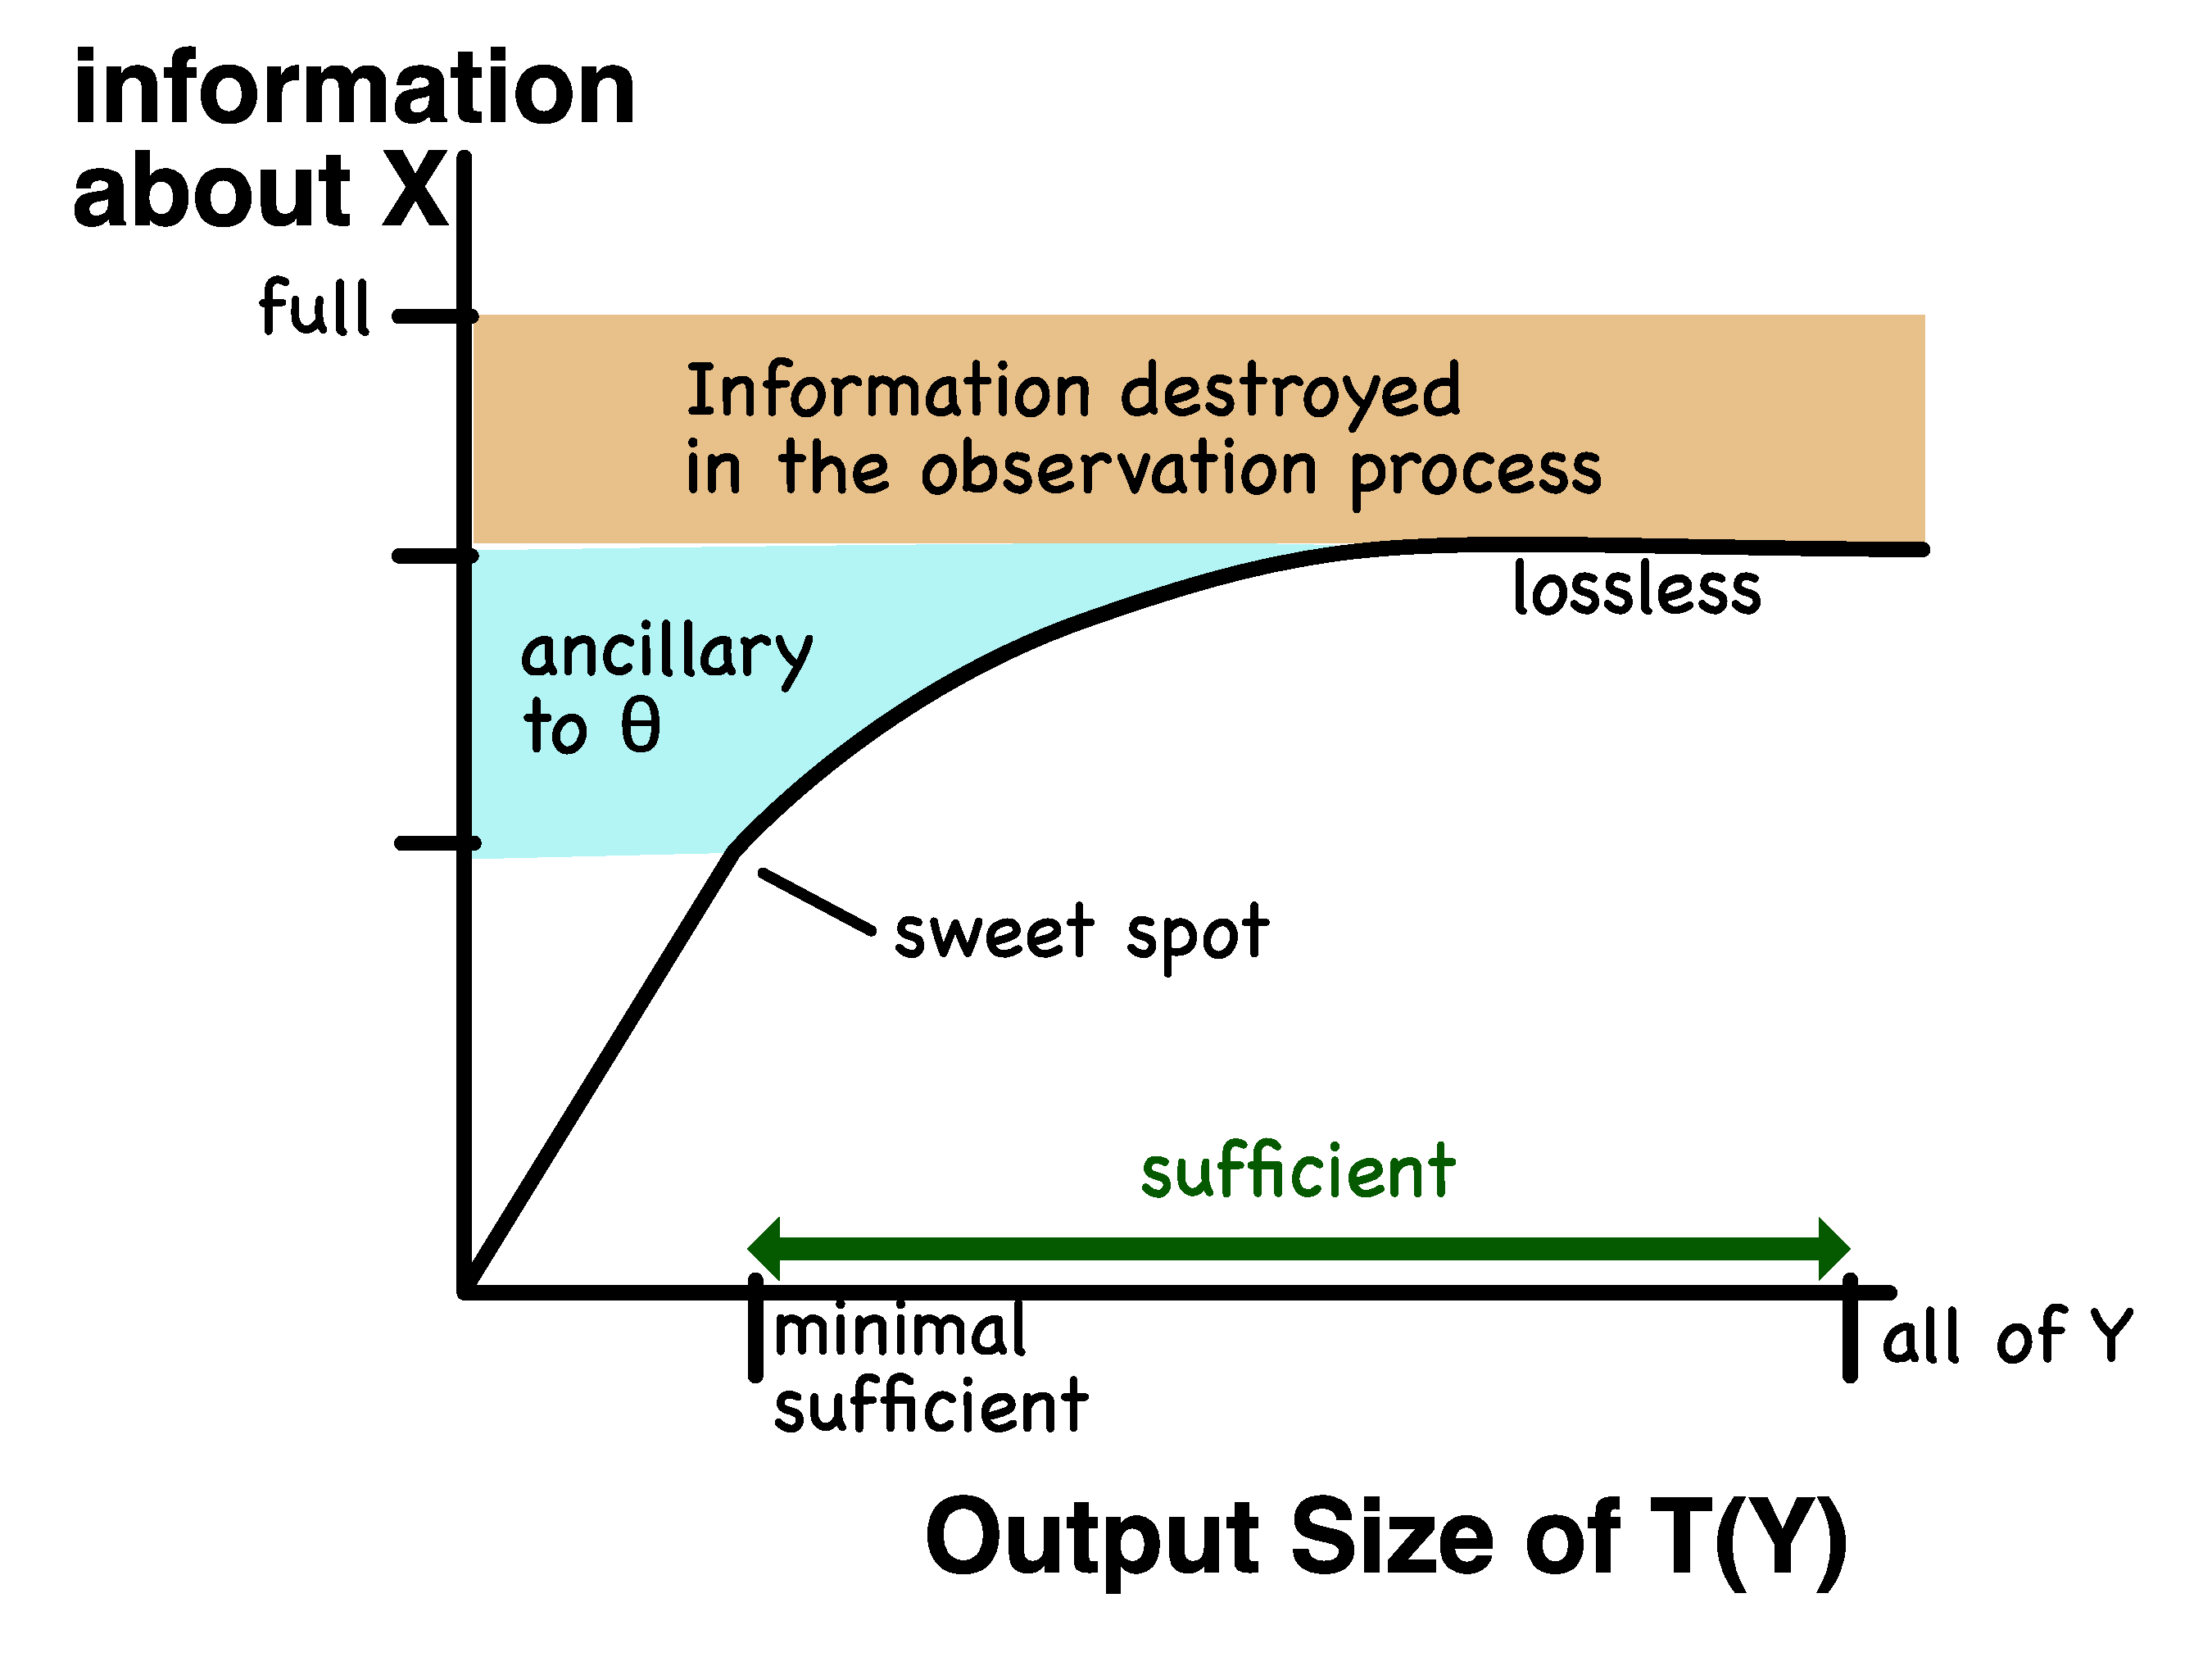
\includegraphics[width=\textwidth]{assets/information.eps}
\end{frame}

\begin{frame}[fragile]
    \frametitle{What should we retain?}
    \begin{itemize}
        \item \textbf{Problem:} The “sweet spot” depends on the scientific model $X \mid \theta$. Different analysts will have different models $X \mid \eta_i$ with a different optimal $T_i\del{Y}$
            \begin{itemize}
                \item and even those might not be known in advance.
            \end{itemize}
        \item \textbf{Goal:} Find a statistic that retains enough information to keep most people happy.
    \end{itemize}
\end{frame}

\begin{frame}[fragile]
    \frametitle{Thank you, but how does one achieve that?}
    \begin{itemize}
        \item involve downstream analysts in the design of preprocessing techniques
    \end{itemize}
\end{frame}

\begin{frame}[fragile]
    \frametitle{Dealing with Nuisance Parameters}

    Researcher conducts $i$ experiments to generate observations $Y_i$, each of which brings a nuisance parameter $\xi_i$. 
    
    % In context of microarray example, each $i$ would be an experiment from one microarray with 
    % its own set of experimental observation parameters
    
    Nuisance parameters present some issues:
    \begin{enumerate}
    \item MLE can be inefficient and inconsistent if $dim(\xi) \to\infty$
    \item Can try and marginalize over the nuisance parameters, but resulting inference can be sensitive to the prior on $\xi$
    \end{enumerate}
    
\end{frame}

\begin{frame}[fragile]

    \frametitle{Regression with Nuisance Parameters: An Example}
    
    \textbf{Sensitivity to nuisance parameters can potentially be eliminated by careful preprocessing}

    \vspace*{5mm}
    
    \textbf{Example:} Select $T$ as a \textbf{partial pivot} so that distribution of $T$ is free of $\xi_2$ for all $\xi_1$ 

    \vspace*{5mm}
    
    \textbf{Data:} $y_{ij} \sim N(\beta_0 + \beta_{1i}x_j, \sigma^2)$ for $j = 1 \ldots m$
    
    \textbf{Downstream analyst wants to estimate:} $\beta_0$ with $\beta_{1i}$ and $\sigma^2$ as nuisance parameters so that $\xi$ = $(\sigma^2, \beta_{11}, ..., \beta_{1n})$
    
\end{frame}

\begin{frame}[fragile]
    \frametitle{Regression with Nuisance Parameters, continued}
   
    \textbf{Preprocessor reduces data to:} $T_i = \frac{1}{m}\sum\del{y_{ij} - \hat{\beta_{ij}}x_j}$ where $\hat{\beta_{1i}}$ is the OLS estimator of $\beta_{1i}$.
    
    \vspace*{5mm}
    
    Distribution of $T_i$ depends on $\sigma^2$ but is free of $B_{1i}$ so $T$ is a partial pivot. 
    
    Reducing $Y$ to $T$ means that only $\xi_1$ is relevant for the distribution of $T$, so inference is more robust to preprocessor's beliefs about $\xi$
    
    % this is since information accumulates on xi_1- we have the same amount of data but one less parameter to estimate. kind of like value functions being "freed up" to perform better estimation %
    
    % Preprocessing that removes nuisance parameters reduces the amount of information available from the data 
    
\end{frame}

\begin{frame}[fragile]
    \frametitle{Preprocessed data -> efficient inference? Really?}

    % Preprocessing is used often to simplify data problems so downstream analysts can apply common methods, so how could it possibly produce efficient inference?
    
    \textbf{Preprocessing allows some assumptions to be more appropriate}:
    
    

\end{frame}

\begin{frame}[fragile]
    \frametitle{Projecting into the future}
    
    \textbf{Likelihood as a minimal sufficient statistic}- computationally efficient approximations of the likelihood function could be foundation for passing information between phases of downstream analysis.  
    
    Two things to consider:
    \begin{enumerate}
    \item Nuisance parameters 
    \item Downstream analysts may be constrained by the likelihood approximation chosen. For example, analysts may want to estimate the data and estimate the parameters, and going from likelihood approximation to estimates of the data, X, could require a lot of effort and computation.
    \end{enumerate}

\end{frame}

\begin{frame}[fragile]
    \frametitle{Projecting into the future}
    
    \textbf{Connection to Multiple Imputation} 
    
    \begin{enumerate}
    \item Relates to prior presentation on congeniality in MI
    \item Both papers want to bound and measure the amount of degradation in inference when information is imperfectly combined
    \item Congeniality paper concludes that nuisance parameters are often a stumbling block for MI, perhaps understanding role of preprocessing in addressing nuisance parameters could be helpful
    \end{enumerate}
    
\end{frame}

\end{document}
